% -*- coding: utf-8 -*-
\documentclass[UTF8,a4paper,10pt]{ctexart}
\usepackage[left=2.54cm, right=2.54cm, top=2.54cm, bottom=2.54cm]{geometry}
\usepackage{amsmath,graphicx,float,booktabs,multirow,enumitem,tikz,pgfplots}
\pgfplotsset{compat=1.17}
\usepackage{ctex}
\setCJKmainfont[ItalicFont=Noto Sans CJK SC Bold, BoldFont=Noto Serif CJK SC Black]{Noto Serif CJK SC}
\usepackage{ctexcap}
\CTEXsetup[name={,、},number={\chinese{section}}]{section}
\CTEXsetup[name={（,）},number={\chinese{subsection}}]{subsection}
\usepackage{fancyhdr}
\pagestyle{fancy}
\lhead{\kaishu \leftmark}
\rhead{\kaishu 并行程序设计实验报告}
\cfoot{\thepage}
\usepackage{xcolor,listings}
\lstset{breaklines,basicstyle=\small,numbers=left,numberstyle=\tiny,frame=trbl}
\usepackage[colorlinks,linkcolor=black,anchorcolor=blue]{hyperref}
\newcommand{\HRule}{\rule{\linewidth}{0.5mm}}

\begin{document}
\begin{titlepage}
\begin{center}
\includegraphics[width=0.8\textwidth]{NKU.png}\\[1cm]
\textsc{\Huge \kaishu{\textbf{南\ \ \ 开\ \ \ 大\ \ \ 学}}} \\[0.9cm]
\textsc{\huge \kaishu{\textbf{计\ 算\ 机\ 学\ 院}}}\\[0.5cm]
\textsc{\Large \textbf{并行程序设计 OpenMP / Pthread 实验报告}}\\[0.8cm]
\HRule \\[0.9cm]
{\LARGE \bfseries ANN 向量检索：OpenMP 与 Pthread 并行优化}\\[0.4cm]
\HRule \\[2.0cm]
\textsc{\LARGE 李华濂}\\[0.5cm]
\textsc{\LARGE 年级: 2024级 \quad 专业: 计算机科学与技术}\\[0.5cm]
\textsc{\LARGE 指导教师: 王刚}\\[0.5cm]
\vfill
{\Large \today}
\end{center}
\end{titlepage}

\newpage
\thispagestyle{empty}
\renewcommand{\abstractname}{\kaishu \sihao \textbf{摘要}}
\begin{abstract}
\noindent 本实验基于 ARM 鲲鹏（Neoverse N1/N2）平台，以 DEEP100K 数据集（100K 底库，96 维，内积距离）为载体，依照指导书评分体系系统探索了 ANN 向量检索中 SIMD NEON 加速与多线程并行优化的组合范式。实验覆盖 Flat-SIMD、PQ-SIMD、IVF-SIMD、IVF-PQ-SIMD和 HNSW五个阶段，各阶段均实现 OpenMP（libgomp）与原生 Pthread（含 atomic fetch\_add 原子分发和线程池）两种并行框架，对每种优化尝试进行了消融实验，并基于 Linux perf 工具进行 IPC、L1/LLC 缓存行为和汇编级热点分析。全文贯穿"索引 $\cdot$ 压缩 $\cdot$ 并行"三层乘积式加速体系与"瓶颈转移定律"的核心方法论。最终 IVF-PQ Pthread FA 框架以 120.5 us/query（Recall 0.963）取得 46.9$\times$ 端到端加速，IVF-SIMD 以 134 us（Recall 0.979）提供低延迟替代方案，HNSW 以 282 us（Recall 0.951, $ef=36$）提供精度约束下的最低延迟方案（$ef$ 可扩展至 64 以 384 us 换取 Recall 0.980）。

\vspace{1em}
\textbf{关键字：} SIMD, NEON, 乘积量化, 倒排索引, HNSW, OpenMP, Pthread, perf 性能分析
\end{abstract}

\tableofcontents
\newpage
\setcounter{page}{1}

%=====================================================================
\section{实验平台与问题概述}
%=====================================================================

\subsection{实验背景}

随着深度学习的发展，图像、文本、音频等非结构化数据被广泛转换为高维向量，最近邻搜索（NNS）在推荐系统、搜索引擎及大语言模型中得到了极为广泛的应用。然而实际工业应用中向量库规模往往达到千万级别且维度通常在 100 维以上，传统精确搜索（暴力计算）复杂度过高。因此，本实验面临的核心问题是：如何构建一个高效的\textbf{近似最近邻搜索（ANNS）系统}，在保持较高 Recall$_{@k}$ 的同时极大降低查询延迟。

ANNS 的核心优化被拆解为两个维度：一是\textbf{减少需要访问的点的数量}——通过 IVF 聚类剪枝、HNSW 图索引等空间划分或图结构，将搜索范围从全库压缩至少量候选；二是\textbf{加快核心底层距离计算速度}——通过 SIMD NEON 向量化（128-bit 一次处理 4 个浮点）和 PQ 乘积量化压缩（将 96 维内积压缩为 4 次查表 + 3 次加法）。本实验在指导书规划的五个阶段中，分别探索多线程并行（OpenMP + Pthread）与上述两类优化的组合范式。
\subsection{实验子问题描述}
本次实验使用OpenMP和Pthread方法对Flat-Simd、PQ-Simd、IVF-Simd、IVF-PQ-Simd与HNSW进行多线程并行优化。
\subsection{实验平台与配置}

\textbf{硬件平台：} ARM 鲲鹏服务器（Neoverse N1/N2 核心），8 核。\textbf{编译器：} GCC -O2。\textbf{数据集：} DEEP100K（100K base + 10K query，向量维度 $d=96$，内积距离度量）。\textbf{评估指标：} 平均延迟（us/query）、Recall$_{@10}$、墙钟加速比、并行效率。\textbf{性能分析工具：} Linux perf（stat / report / annotate）。\textbf{并行框架：} OpenMP（libgomp 运行时）与原生 Pthread（含 atomic fetch\_add 原子分发）。

%=====================================================================
\section{Flat-SIMD 多线程并行}
%=====================================================================

\subsection{算法与并行策略}

Flat-SIMD 是暴力最近邻搜索的 NEON 加速版：对每条 Query，计算其与全部 100K 底库向量的内积距离，从 100K 个距离中选出最小的 $k=10$ 个。核心距离函数 \texttt{InnerProductSIMDNeon} 利用 ARM NEON \texttt{float32x4\_t} 128-bit 寄存器一次处理 4 个浮点数，\texttt{vmlaq\_f32} 融合乘加指令（FMA）在单周期内完成 $a \times b + c$，双累加器交替使用以隐藏 FMA 延迟（ILP=2）。

\textbf{并行策略：单 Query 内部 Base 划分并行。} 将 100K 底库按 \texttt{schedule(static)} 均匀切分给各线程，每线程维护私有局部 TopK 堆（容量 $k=10$），计算结束后通过 \texttt{\#pragma omp critical} 一次性合并。选择 intra-query 而非外层 Query 级并行的原因是：Flat-SIMD 为 compute-bound 场景，每条 Query 的计算量足够大（100K $\times$ 96 维 NEON 内积 $\approx$ 5600 us），可支撑多核分摊。

\begin{lstlisting}[language=C++, caption={Flat-SIMD intra-query 底库划分并行 (main.cc)}]
inline std::priority_queue<std::pair<float, int>> flat_simd_omp_search(
    const float* base, const float* query, size_t base_number,
    size_t vecdim, size_t k, int num_threads)
{
    std::priority_queue<std::pair<float, int>> global_topk;
    #pragma omp parallel num_threads(num_threads)
    {
        std::priority_queue<std::pair<float, int>> local_topk;
        #pragma omp for schedule(static)         // 底库均匀切分, 无负载不均
        for (size_t i = 0; i < base_number; ++i) {
            float dist = InnerProductSIMDNeon(query, base + i * vecdim, vecdim);
            if (local_topk.size() < k) local_topk.push({dist, (int)i});
            else if (dist < local_topk.top().first)
                { local_topk.pop(); local_topk.push({dist, (int)i}); }
        }
        #pragma omp critical                      // 局部堆合并到全局堆
        { while (!local_topk.empty()) { global_topk.push(local_topk.top());
            local_topk.pop();
            if (global_topk.size() > k) global_topk.pop(); } }
    }
    return global_topk;
}
\end{lstlisting}

\textbf{设计要点：}\texttt{schedule(static)}——所有 SIMD 内积计算量完全一致（96 维 $\times$ 固定条数），无负载不均问题；局部堆容量仅 $k=10$，push/pop 开销 $O(\log k)$ 可忽略；合并阶段仅处理 $threads \times k$ 个元素，critical 区极短。\textbf{Pthread 版本}采用等同逻辑，手工 \texttt{pthread\_create/join} + static 均分替代 OpenMP fork-join，核心计算循环完全一致。

\subsection{实验结果}

\begin{table}[H]
\centering
\caption{Flat-SIMD 多线程消融实验结果（Recall = 0.99999）}
\begin{tabular}{cccccc}
\hline
线程数 & 1 & 2 & 4 & 8 & 理想 \\
\hline
延迟 (us) & 5646 & 2799 & 1552 & 1015 & 706 \\
加速比 & 1.00× & 2.02× & 3.64× & 5.56× & 8.00× \\
并行效率 & 100\% & 101\% & 91\% & 70\% & 100\% \\
\hline
\end{tabular}
\end{table}

\begin{figure}[H]
\centering
\begin{tikzpicture}
\begin{axis}[width=0.85\textwidth,height=5.5cm,xlabel={线程数},ylabel={加速比},grid=major,
    legend style={at={(0.02,0.98)},anchor=north west}]
\addplot[color=blue,mark=*,thick] coordinates {(1,1.00)(2,2.02)(4,3.64)(8,5.56)};
\addplot[color=gray,mark=triangle*,dashed,thick] coordinates {(1,1)(2,2)(4,4)(8,8)};
\legend{实测加速比, 理想加速比 ($y=x$)}
\end{axis}
\end{tikzpicture}
\caption{Flat-SIMD 加速比曲线。2 线程轻微超线性（2.02×，效率 101\%），8 线程 5.56×，效率 70\%。}
\end{figure}

\textbf{关键观察：}
\begin{itemize}
\item 2 线程出现超线性加速（2.02×，效率 101\%），归因于 L1 Cache 工作集拆分效应——2 线程各处理 50K 向量，每线程 L1 压力减半，Cache 命中率提升的微幅收益超出线程调度开销。
\item 4→8 线程效率从 91\% 降至 70\%，衰减主因：critical 区合并的 Amdahl 串行瓶颈（8 线程排队合并 80 个元素）和共享内存带宽竞争。
\end{itemize}

\subsection{性能分析}

\begin{table}[H]
\centering
\caption{Flat-SIMD 单核 Baseline perf stat}
\begin{tabular}{lc}
\hline
指标 & 数值 \\
\hline
cpu-cycles & 621.4 G \\
instructions & 1102.3 G \\
\textbf{IPC} & \textbf{1.77} \\
L1-dcache-loads & 312.0 G \\
L1 miss rate & 1.50\% \\
LLC miss rate & 12.81\% \\
\hline
\end{tabular}
\end{table}

IPC = 1.77 表明 NEON 内积的流式连续访存行为优良，CPU 超标量流水线得到充分利用。L1 miss 率 1.50\% 验证了顺序扫描 base 向量的高 cacheline 利用率（每条 96 维 $\times$ 4B = 384B，跨 6 个 cacheline，顺序预取有效）。Flat-SIMD 作为 compute-bound 基准，为后续 PQ-SIMD 的 memory-bound 并行行为提供对照基线。

\subsection{Pthread 版本：四种并行模式与 top-p 权衡实验}

指导书指出 Flat-SIMD 并行可考虑"query 级并行或者 base 向量划分并行（此时需考虑 topk 的 reduce，因此每个线程求出的 top p 中 p 的取值也会影响 recall 和 latency 的 trade-off）"。为系统探索这一设计空间，Pthread 版本实现了四种并行模式和一个参数化实验。

\subsubsection{四种并行模式设计}

\textbf{IntraStatic（底库静态均分）：} 将 100K 底库按 static 均分给各线程，每线程维护容量为 $p$ 的局部堆，最后 \texttt{heap\_merge} 合并至全局 TopK。对标 OpenMP 版本的 \texttt{schedule(static)} 策略。

\textbf{IntraDynamic（底库原子竞争）：} 各线程通过 \texttt{atomic<size\_t>::fetch\_add(1)} 动态抢占底库向量索引。设计初衷是解决潜在负载不均（虽然 Flat-SIMD 中每次内积计算量严格一致，但在 NUMA 或异构核心上可能产生差异）。预期因 per-vector 原子竞争开销过大而呈负优化。

\textbf{InterStatic / InterDynamic（Query 级并行）：} 外层 Query 均分或原子分发，内层每线程独立执行纯串行搜索。对标后续所有章节中确证为最优的 Inter-Query 批量并发范式。

\subsubsection{top-p 参数对延迟的影响实验}

$p$（每线程局部堆大小）是 Flat-SIMD 并行中控制 recall--latency 的调节旋钮。在精确距离场景下，$p$ 不影响 Recall（所有距离均为精确 NEON 内积），但通过堆操作的 $O(\log p)$ 复杂度影响延迟。在近似距离场景（如后续的 PQ ADC），$p$ 过小会导致被 ADC 误差挤出的真近邻丢失，Recall 下降。

\begin{table}[H]
\centering
\caption{IntraStatic 模式 $p$ 值扫描 —— 延迟影响（4 线程, $k=10$, Recall=0.99995）}
\begin{tabular}{cccccc}
\hline
$p$ & $k$ (10) & $2k$ (20) & $5k$ (50) & $10k$ (100) & $20k$ (200) \\
\hline
延迟 (us) & 2295 & 2410 & 2370 & 2510 & 2412 \\
vs $p=k$ 开销增幅 & — & +5.0\% & +3.3\% & +9.4\% & +5.1\% \\
\hline
\end{tabular}
\end{table}

\textbf{关键发现：} 在精确距离（Flat-SIMD）场景下，$p$ 从 $k$ 增至 $20k$（200× 增长），延迟仅增加 $\sim$5--9\%，无统计显著的上升趋势。这是因为 $k=10$ 的小堆使得 push/pop 的 $O(\log p)$ 差异被 NEON 内积的 $O(d)$ 计算量（$\sim$0.6 us/条）充分稀释。\textbf{然而在近似距离场景（PQ ADC）中，$p$ 的影响将截然不同——ADC 的近似误差需要 $p \gg k$ 来提供"缓冲区"以防止真近邻被挤出局部堆}，这一机制在 PQ-SIMD 章节的 $P_{size}=2500$ 设计中得到了应用。

\subsubsection{IntraDynamic：原子竞争的负优化实证}

\begin{table}[H]
\centering
\caption{IntraDynamic 模式线程扩展实验结果（$p=k=10$, Recall=0.99995）}
\begin{tabular}{ccccc}
\hline
线程数 & 1 & 2 & 4 & 8 \\
\hline
延迟 (us) & 6761 & 9233 & 16936 & 24761 \\
加速比 & 1.00× & \textbf{0.73×} & \textbf{0.40×} & \textbf{0.27×} \\
\hline
\end{tabular}
\end{table}

IntraDynamic 在所有线程数下均表现为严重负优化，且随线程数增加呈超线性劣化（8c 延迟是 1c 的 3.7 倍）。根因在于：100K 次 \texttt{fetch\_add}（每次编译为 \texttt{ldxr / add / stxr / cbnz} 四条指令的 lock-free CAS 循环）在 8 线程并发下产生极高的 cacheline 乒乓（ping-pong）开销——原子变量所在 cacheline 在 8 个核心的 L1 之间反复无效化-重载，每次 CAS 重试导致 $\sim$20--50 cycles 的额外延迟。\textbf{该案例定量定义了原子竞争的适用边界：仅当单任务计算量远大于原子操作开销（$\frac{T_{\text{comp}}}{T_{\text{atomic}}} \gg 1$）时，per-element 原子分发才有正向收益。} Flat-SIMD 中每向量仅 $\sim$0.6 us 的 NEON 内积显然不满足此条件。与之对比，后续 IVF/IVF-PQ/HNSW 中 per-query 的原子分发（$\frac{T_{\text{query}}}{T_{\text{atomic}}} \sim 10^4$--$10^5$）则完全无此问题。

\subsubsection{InterDynamic：批量并行的最优选择}

\begin{table}[H]
\centering
\caption{InterDynamic 模式线程扩展实验结果（Recall=0.99995）}
\begin{tabular}{cccccc}
\hline
线程数 & 1 & 2 & 4 & 8 & 理想 \\
\hline
墙钟 (ms) & 13944 & 5642 & 3432 & 2012 & — \\
avg\_lat (us) & 6972 & 2821 & 1716 & 1006 & — \\
加速比 & 1.00× & 2.47× & 4.06× & \textbf{6.93×} & 8× \\
\hline
\end{tabular}
\end{table}

InterDynamic 以 6.93× 加速比成为 Flat-SIMD Pthread 版本的最优模式。与 OpenMP intra-query 版本（5.56×）相比，Pthread 的 Inter-Query 批量并发额外获得了 1.25× 的加速收益。这一优势的来源与 IVF-SIMD 尝试三的机制相同：将并行边界从"Query 内部"提升至"Query 之间"后，所有 intra-query 的 critical 区同步被彻底消除，仅余外层 \texttt{pthread\_join} 的隐式汇合点作为唯一的串行分量。8 线程加速比 6.93×（效率 86.6\%）显著高于 OpenMP intra-query 的 5.56×（效率 69.5\%）。

\subsubsection{Flat-SIMD OpenMP vs Pthread 双架构对比}

\begin{table}[H]
\centering
\caption{Flat-SIMD OpenMP vs Pthread 四模式对比总结}
\begin{tabular}{lccc}
\hline
模式 & 框架 & 策略 & 最佳加速比 \\
\hline
Intra-Static & OpenMP & \texttt{schedule(static)} + critical merge & 5.56× (8c) \\
Intra-Static & Pthread & static 均分 + heap\_merge & 3.59× (4c), 8c 负优化(3.22×) \\
Intra-Dynamic & Pthread & per-vector fetch\_add 原子竞争 & \textbf{0.27× (8c)} — 严重负优化 \\
Inter-Dynamic & Pthread & per-query fetch\_add 批量分发 & \textbf{6.93× (8c)} — \textbf{Flat 阶段最优} \\
\hline
\end{tabular}
\end{table}

\textbf{Flat-SIMD 阶段核心结论：} (1) Inter-Query 批量并发（Pthread InterDynamic, 6.93×）优于 Intra-Query 底库划分（OpenMP, 5.56×）(2) top-p 参数在精确距离场景中影响微乎其微（$<$10\%），但在后续 PQ-SIMD 近似场景中可能成为 recall 的影响因素；(3) per-element 原子竞争（IntraDynamic）在此 compute-light 场景中为负优化，定义了原子分发粒度的下界——\textbf{原子操作适用于任务级（per-query）分发而非数据级（per-vector）分发。}

\begin{table}[H]
\centering
\caption{Flat-SIMD Pthread perf stat（全模式联合运行）}
\begin{tabular}{lc}
\hline
指标 & 数值 \\
\hline
IPC & 0.86 \\
L1 miss rate & 1.68\% \\
context-switches & 0 \\
cpu-migrations & 0 \\
inter\_dynamic\_worker & 60.60\%（批量 Query 主导） \\
intra\_static\_worker & 38.34\% \\
\hline
\end{tabular}
\end{table}

%=====================================================================
\section{PQ-SIMD 多线程优化}
%=====================================================================

\subsection{算法原理}

乘积量化（Product Quantization, PQ）是 ANNS 中压缩距离计算的核心技术。训练流程：(1) 将 96 维向量等分为 $M=4$ 个子空间（每子空间 $d_{sub}=24$ 维）；(2) 对每个子空间独立运行 K-Means 聚类（$K_{pq}=256$ 个中心，8-bit 编码），得到 4 组 Codebook（每组 256 个 24 维质心）；(3) 将每条底库向量编码为 4 字节的 PQ code（每字节 = 该子空间最近质心索引）。

在线查询的 ADC（Asymmetric Distance Computation）阶段，距离计算从 96 次浮点乘加压缩为 4 次查表 + 3 次加法：先构建 4 张 LUT（$4 \times 256 \times 4 = 4$KB），每条向量的近似距离 = LUT[0][code[0]] + LUT[1][code[1]] + LUT[2][code[2]] + LUT[3][code[3]]。计算量降低约 48×，代价是访存模式从连续流式变为伪随机 LUT 跳转。

\begin{lstlisting}[language=C++, caption={PQ 训练 —— 子空间 K-Means (pq\_train.h)}]
inline void train_pq(const float* base, size_t N, size_t d, int M, int K,
                     std::vector<float>& codebooks) {
    size_t sub = d / M; int max_iter = 15;
    for (int m = 0; m < M; ++m) {
        // 随机初始化聚类中心
        float* cent = &codebooks[m * K * sub];
        for (int k = 0; k < K; ++k)
            memcpy(cent + k * sub, base + (rand()%N) * d + m * sub, sub*4);
        // 迭代 K-Means (OpenMP 加速 assign)
        std::vector<int> assign(N);
        for (int iter = 0; iter < max_iter; ++iter) {
            #pragma omp parallel for
            for (size_t i = 0; i < N; ++i) { /* 找最近中心... */ }
            // 主线程更新质心...
        }
    }
}
\end{lstlisting}

\subsection{OpenMP 版本：两种并行策略}

\textbf{策略 A —— Pthread 风格静态分块扫描}（\texttt{pq\_adc\_search\_chunk\_parallel}）：主线程串行构建 4 张 LUT（开销 $<$ 25 us），然后创建线程各负责底库的一段（static 均分），无锁写入共享 \texttt{dist\_array}。主线程统一执行 \texttt{nth\_element}（$O(N)$）选 top-$P_{size}$ 候选，最后仅对候选集 SIMD 精排。\textbf{以 nth\_element 替代初版中局部堆 + critical 合并的低效范式}。

\begin{lstlisting}[language=C++, caption={策略 A：无锁静态分块 + nth\_element 选优 (pq\_train.h)}]
std::vector<std::pair<float,int>> dist_array(N);
#pragma omp parallel
{   int tid = omp_get_thread_num(), nth = omp_get_num_threads();
    size_t chunk = N / nth, s = tid * chunk;
    size_t e = (tid == nth-1) ? N : s + chunk;
    for (size_t i = s; i < e; ++i) {
        auto p = pq_base + i * M;
        float dot = lut[0][p[0]]+lut[1][p[1]]+lut[2][p[2]]+lut[3][p[3]];
        dist_array[i] = {1.0f - dot, (int)i};
    }
}
std::nth_element(dist_array.begin(), dist_array.begin()+P_size, dist_array.end());
// 仅对 P_size 条候选进行 InnerProductSIMDNeon 精排
\end{lstlisting}

\textbf{策略 B —— 批量 Query 并发}：外层 \texttt{parallel for schedule(dynamic)} 对 2000 条 Query 并发，内层调用完全无锁的纯串行 ADC 管线 \texttt{pq\_adc\_search\_pure\_serial}。

\begin{lstlisting}[language=C++, caption={策略 B：纯串行 ADC 内层（专供 Batch Query 并发调用）}]
inline auto pq_adc_search_pure_serial(...) {
    float lut[4][256];
    for (int m = 0; m < M; ++m) {                  // 串行构建 4 张 LUT
        auto sq = query + m * sub;
        auto cb = codebooks_SoA.data() + m * K_pq * sub;
        for (int c = 0; c < K_pq; ++c) { float d=0;
            for (size_t j=0; j<sub; ++j) d += sq[j] * cb[j * K_pq + c];
            lut[m][c] = d; }
    }
    std::vector<std::pair<float,int>> da(N);       // 扁平数组, 零堆操作
    for (size_t i=0; i<N; ++i) { auto p=pq_base+i*M;
        da[i]={1.0f-(lut[0][p[0]]+lut[1][p[1]]+lut[2][p[2]]+lut[3][p[3]]),(int)i}; }
    std::nth_element(da.begin(), da.begin()+P_size, da.end());
    std::priority_queue<...> fine;                 // SIMD 精排 top-K
    for (size_t i=0; i<P_size; ++i) { /* InnerProductSIMDNeon reranking */ }
    return fine;
}
#pragma omp parallel for schedule(dynamic)
for (int i = 0; i < test_number; ++i)
    results[i] = pq_adc_search_pure_serial(pq_base, base, queries+i*d, N, d, k, ...);
\end{lstlisting}

\subsection{Pthread 版本：两种策略的原子分发替代}

\textbf{策略 A（Pthread）—— intra-query 底库分块}：\texttt{pthread\_create} $nthreads$ 个 worker 各负责底库 static 均分段，无锁写入共享 \texttt{dist\_array}，主线程 \texttt{pthread\_join} 后统一 \texttt{nth\_element} 和精排。

\textbf{策略 B（Pthread）—— inter-query 原子分发}：主线程一次性创建 $nthreads$ 个 Pthread，worker 通过 \texttt{atomic<size\_t>::fetch\_add(1)} 自取 Query 索引，内部执行完整串行 ADC 管线，零线程间交互。

\begin{lstlisting}[language=C++, caption={Pthread 策略 B：atomic fetch\_add 零互斥分发 (pq\_pthread.h)}]
static void* batch_worker(void* arg) {
    BatchArg* a = (BatchArg*)arg;
    while (true) {
        size_t i = a->next->fetch_add(1, std::memory_order_relaxed);
        if (i >= a->query_n) break;
        auto q = a->queries + i * a->vecdim;
        float lut[4][256]; pq_build_lut(q, a->sub_dim, a->M, a->K_pq, *a->cb, lut);
        std::vector<std::pair<float,int>> da(a->N);   // 串行 ADC
        for (size_t j=0; j<a->N; ++j) { auto p=a->pq+j*a->M;
            da[j]={1.0f-(lut[0][p[0]]+lut[1][p[1]]+lut[2][p[2]]+lut[3][p[3]]),(int)j}; }
        std::nth_element(da.begin(), da.begin()+a->P, da.end());
        std::priority_queue<...> fine; /* SIMD reranking + recall */
    }
    return nullptr;
}
\end{lstlisting}

\subsection{实验结果与性能分析}

\begin{table}[H]
\centering
\caption{PQ-SIMD OpenMP vs Pthread 实验结果汇总（Recall=0.976）}
\begin{tabular}{cccccc}
\hline
\multirow{2}{*}{线程} & \multicolumn{2}{c}{OpenMP 策略 A（分块）} & \multicolumn{2}{c}{Pthread 策略 B（墙钟）} & 理想 \\
& 延迟(us) & 加速比 & 墙钟(ms) & 加速比 & \\
\hline
1 & 1700.2 & 1.00× & 3607.2 & 1.00× & 1× \\
2 & 1590.6 & 1.07× & 1817.2 & 1.98× & 2× \\
4 & 1424.7 & 1.19× & 890.4  & 4.05× & 4× \\
8 & 1411.5 & \textbf{1.20×} & 515.3  & \textbf{7.00×} & 8× \\
\hline
\end{tabular}
\end{table}

\begin{figure}[H]
\centering
\begin{tikzpicture}
\begin{axis}[width=0.8\textwidth,height=5.5cm,xlabel={线程数},ylabel={延迟 (us) / 加速比},ybar,bar width=10pt,xtick=data,
    legend style={at={(0.5,-0.22)},anchor=north,legend columns=-1}]
\addplot coordinates {(1,1700.2)(2,1590.6)(4,1424.7)(8,1411.5)};
\addplot coordinates {(1,1607.3)(2,1608.6)(4,1678.4)(8,1727.7)};
\legend{策略 A (Chunk 扫描), 策略 B (Batch Query per-query 计时)}
\end{axis}
\end{tikzpicture}
\caption{PQ-SIMD 两种策略延迟对比。策略 A 微弱正加速 1.20×，策略 B per-query 计时出现负优化（内存带宽饱和）。}
\end{figure}

\textbf{核心发现——测量方法论决定结论方向：} OpenMP 策略 A（intra-query）仅获 1.20×，策略 B per-query 计时呈现负优化（0.93× @ 8c，因多核共享内存带宽竞争拖慢单条计时窗口）。但 Pthread 策略 B 墙钟度量展现 7.00× 吞吐加速——同一算法逻辑，per-query 计时含并发竞争噪声，墙钟反映真实系统吞吐。\textbf{PQ-SIMD 的优化目标应定为 QPS 吞吐而非 per-query 延迟。}

\begin{table}[H]
\centering
\caption{PQ-SIMD perf 与双架构对比}
\begin{tabular}{lcc}
\hline
指标 & OpenMP 策略 A (8c) & Pthread (策略A+B 联合) \\
\hline
IPC & $\sim$1.0 (严重 stall) & 1.74 (内存延迟掩盖) \\
L1 miss rate & — & 0.57\% \\
ctx-switch / migration & — & 0 / 0 \\
热点指令 & \texttt{ldr s0} 34.51\% & \texttt{ldr s2} 54.91\% + \texttt{ldrb w5} 44.87\% \\
计算/访存周期比 & $\approx$3.86 & $\approx$0.0005 (计算指令$<$0.05\%) \\
\hline
\end{tabular}
\end{table}

\textbf{物理瓶颈确证：} ADC 的 4 路伪随机 LUT 查表将系统锁死在 memory-bound——访存指令（4×ldrb + 4×ldr）占 $\sim$99.8\% 周期，浮点计算 $<$ 0.05\%。L1 miss 率 0.57\% 证实 4KB LUT 几乎全程驻留 L1D，但即使完美命中，100K $\times$ 4 次 LDR 的理论下界 $\sim$1000 us 已接近实测 1800 us。\textbf{并行上限被 L1 私有性和 load port 数量不可逆锁死，intra-query 优化空间 $\le$1.20×。}

\textbf{汇编级取证——内存墙的两条铁证：}

\begin{lstlisting}[language={[x86masm]Assembler}, caption={OpenMP 策略 A 热点汇编：标量 LUT 查表主导}]
Percent│      ldrb w5, [x0, #2]           // 加载 PQ code byte (3.67%)
  3.78 │      ldr  s3, [x4, x6, lsl #2]   // LUT[0][code0]  (3.78%)
 34.51 │      ldr  s0, [x4, x7, lsl #2]   // �� LUT 查表占 34.51% —— 单条指令!
 10.38 │      ldr  s2, [x4, x5, lsl #2]   // LUT[2][code2] (10.38%)
  9.28 │      ldr  s1, [x4, x3, lsl #2]   // LUT[3][code3] (9.28%)
       │      fadd s0, s0, s3             // 累加 (< 0.01%)
 13.58 │      fsub s0, s4, s0             // 1.0-dot  (< 0.01%)
\end{lstlisting}

4 次 LUT 查表合计占 \textbf{57.95\%} 的 CPU 周期，而真正的浮点计算（fadd + fsub）合计不足 15\%。$\frac{\text{访存周期}}{\text{计算周期}} \approx 3.86$。Pthread 版本的 intra\_chunk\_worker 汇编进一步将这一比例推向极致：\texttt{ldrb w5}（44.87\%）+ \texttt{ldr s2}（54.91\%）几乎平分全部周期，4 次 LUT 查表 + 4 次 code byte 加载合计 \textbf{99.8\%}，浮点指令的采样率低于 perf 的统计噪声阈值。

\textbf{为什么 OpenMP 策略 B per-query 计时呈负优化？} 当 8 个线程同时执行独立的串行 ADC 时，每条 Query 的 per-query 计时窗口（\texttt{gettimeofday} 对）包含了：(i) 自身上下文中的 100K 次 LUT 查表（$\sim$1600 us 纯计算）；(ii) 另外 7 个线程对共享内存总线、LLC 和 L2 缓存的并发争用产生的额外排队延迟——该延迟在单条计时的统计均值中表现为线性叠加。墙钟度量则不含此竞争噪声，因为它只记录最早开始和最晚完成的时间戳差。\textbf{两种度量在 memory-bound 场景下给出相反的"优化/负优化"判定——这是本实验最具方法论价值的发现之一。}

\begin{table}[H]
\centering
\caption{PQ-SIMD OpenMP vs Pthread 并行策略全览}
\begin{tabular}{lccc}
\hline
策略 & 框架 & 实现方式 & 最佳加速比 \\
\hline
策略 A（底库分块） & OpenMP & omp parallel + tid 切分 + nth\_element & 1.20× (8c) \\
策略 A（底库分块） & Pthread & pthread\_create + static 均分 & 0.94× (8c, 含线程创建) \\
策略 B（Batch Query） & OpenMP & \texttt{parallel for schedule(dynamic)} & 0.93× (per-query) \\
策略 B（Batch Query） & Pthread & atomic fetch\_add 零互斥 & \textbf{7.00×} (墙钟吞吐) \\
\hline
\end{tabular}
\end{table}

%=====================================================================
\section{IVF-SIMD 多线程优化}
%=====================================================================

\subsection{算法原理与 Baseline 实现}

IVF（Inverted File Index）通过 K-Means 聚类（$K_{ivf}=1000$）将底库划分到 1000 个簇，查询时采用粗到细两阶段：(1) \textbf{粗排}——计算 Query 与 1000 个簇中心的 SIMD 内积距离，选出最近 $nprobe=50$ 个簇；(2) \textbf{精排}——扫描这 50 个簇内的全部底库向量，用 SIMD 算真实内积距离，取全局 TopK。相比 Flat-SIMD 的全库 100K 暴力扫描，IVF 将搜索空间压缩至约 5K（$nprobe \times$ 平均簇人数），实现 7.1× 算法加速。

\subsubsection{纯串行 Baseline}

\begin{lstlisting}[language=C++, caption={IVF-SIMD 纯串行 Baseline (IVF-baseline.cc)}]
inline auto ivf_simd_baseline_search(
    const vector<float>& centroids, const vector<IVFList>& lists,
    const float* base, const float* query, size_t d, size_t k, int nprobe)
{
    int K_ivf = centroids.size() / d;
    // 阶段 1: 粗排 —— 1000 次 SIMD 内积, 找最近 nprobe 个簇
    std::priority_queue<std::pair<float,int>> coarse;
    for (int c = 0; c < K_ivf; ++c) {
        float dist = InnerProductSIMDNeon(query, centroids.data() + c * d, d);
        if (coarse.size() < nprobe) coarse.push({dist, c});
        else if (dist < coarse.top().first) { coarse.pop(); coarse.push({dist, c}); }
    }
    // 阶段 2: 精排 —— 扫描选中的 nprobe 个簇内的所有向量
    std::priority_queue<std::pair<float,int>> fine;
    while (!coarse.empty()) { int cid = coarse.top().second; coarse.pop();
        for (int vid : lists[cid].ids) {
            float d = InnerProductSIMDNeon(query, base + vid * d, d);
            if (fine.size() < k) fine.push({d, vid});
            else if (d < fine.top().first) { fine.pop(); fine.push({d, vid}); }
        }
    }
    return fine;
}
\end{lstlisting}

\begin{table}[H]
\centering
\caption{IVF-SIMD Baseline 实验结果与 perf stat}
\begin{tabular}{lcc}
\hline
指标 & 数值 & 对比 Flat-SIMD \\
\hline
延迟 & 795 us & 7.1× 加速 \\
Recall$_{@10}$ & 0.97884 & 损失 2.1\% \\
IPC & 1.77 & 持平 \\
L1 miss rate & 1.50\% & 持平 \\
LLC miss rate & 12.81\% & 持平 \\
\hline
\end{tabular}
\end{table}

\subsection{OpenMP 优化：三个递进尝试}

\subsubsection{尝试一 —— 粗排阶段并行（负向优化）}

\textbf{策略：} 对粗排的 1000 次 SIMD 内积使用 \texttt{schedule(static)} 并行，各线程维护局部堆，\texttt{critical} 合并。精排保持串行。

\textbf{结果：} 1c=852 us, 2c=808 us, 4c=813 us, 8c=\textbf{928 us}（加速比 \textbf{0.92×} $<$ 1.0，负优化）。Recall 恒定 0.97884。

\textbf{原因：} 粗排仅需 1000 次 SIMD 内积（单线程 $\sim$30 us），远小于 OpenMP fork-join + critical 合并开销之和（$\sim$50--80 us），计算--开销比严重倒挂。

\textbf{perf report 的量化（8 线程）：}\texttt{train\_ivf} 75.31\%（离线训练），\texttt{libgomp.so} 内部函数合计 $\sim$14\%（含 \texttt{GOMP\_parallel}、\texttt{GOMP\_critical\_start}、\texttt{GOMP\_barrier} 等），而搜索核心 \texttt{search\_attempt1\_coarse\_parallel} 仅占 \textbf{5.02\%}——OpenMP 运行时开销（14\%）是实际搜索计算（5\%）的近 3 倍。perf annotate 进一步揭示：\texttt{train\_ivf} 内层循环中 \texttt{cmp x2, x0}（65.52\%）+ \texttt{ldr s2}（20.02\%）的 L2 距离计算循环主导了训练阶段的耗时——但这些周期与在线查询完全无关。该案例定量定义了并行化的计算量下界：在 ARM NEON 平台上，单任务 SIMD 内积计算量需 $\gtrsim$ 5000 次（对应 $\sim$0.5 ms）方能有效利用多核并行。

\subsubsection{尝试二 —— 精排阶段并行（正向优化）}

\textbf{策略：} 粗排保持串行，对 $nprobe=50$ 个簇的倒排表扫描使用 \texttt{schedule(dynamic, 1)} 并行。\textbf{dynamic 是核心}——K-Means 产生的簇大小天然非均匀（50--300 人/簇），\texttt{static} 调度将导致"大簇"线程长尾瓶颈，\texttt{dynamic,1} 以单簇粒度动态分配实现自动负载均衡。

\begin{lstlisting}[language=C++, caption={尝试二：精排簇并行 —— schedule(dynamic,1) 关键设计}]
std::priority_queue<std::pair<float,int>> global_topk;
#pragma omp parallel
{
    std::priority_queue<std::pair<float,int>> local_topk;
    #pragma omp for schedule(dynamic, 1)        // 核心: dynamic 解决非均匀簇!
    for (size_t i = 0; i < selected.size(); ++i) {
        for (int vid : lists[selected[i]].ids) {
            float d = InnerProductSIMDNeon(query, base + vid * d, d);
            if (local_topk.size() < k) local_topk.push({d, vid});
            else if (d < local_topk.top().first)
                { local_topk.pop(); local_topk.push({d, vid}); }
        }
    }
    #pragma omp critical { /* 合并局部 TopK 到 global_topk */ }
}
\end{lstlisting}

\textbf{结果：} 1c=896 us, 2c=446 us, 4c=321 us, 8c=\textbf{221 us}（加速比 \textbf{4.05×}）。Recall 恒定 0.97884。

\textbf{成功原因：} 精排计算量充足（$\sim$5000 次 96 维 SIMD 内积，单线程 $\sim$800 us），8 线程每线程仍承担 $\sim$6 簇 $\approx$ 600 次 SIMD 内积（$\sim$100 us 纯计算），远超调度开销（$\sim$10--20 us）。2 线程轻微超线性（2.01×），Cache 工作集拆分效应再现——2 线程各处理约 2500 个向量的内积，每线程 L1/L2 Cache 压力减半。

\textbf{从正优化到亚线性的衰减机制分析：} 4→8 线程效率从 69.8\% 降至 50.7\%，加速比仅从 2.79× 增至 4.05×（4→8 额外加速 1.45×，理想为 2.0×）。衰减的双重根因：(i) \texttt{\#pragma omp critical} 合并阶段构成 Amdahl 串行瓶颈——8 线程在 critical 区外排队，排队线程数随核心数增加而增长；(ii) 每线程的纯计算量从 4 线程时的 $\sim$12 簇（$\sim$200 us）降至 8 线程时的 $\sim$6 簇（$\sim$100 us），计算--开销比从 $\sim$10:1 缩至 $\sim$5:1，调度开销的相对权重翻倍。

\textbf{perf stat 佐证（8 线程精排并行单次运行）：} IPC 1.95（接近 Flat-SIMD 的 1.77），L1 miss 1.49\%，LLC miss 7.69\%——纯 SIMD 内积的流式访存未因并行引入额外 Cache 竞争。但总 cpu-cycles（623.6G $\to$ 755.6G，+21\%）的增量全数源于线程调度和 critical 合并的系统开销——这 21\% 的"并行税"在 4.05× 的墙钟加速面前被充分覆盖，但在 8 线程时已明显拖累边际收益。

\subsubsection{尝试三 —— Query 级批量并行（最优方案）}

\textbf{策略：} 将并行边界从"Query 内部"提升至"Query 之间"。外层 \texttt{parallel for schedule(dynamic)}，内层每条 Query 独立执行纯串行 IVF 搜索（\texttt{serial\_baseline}），彻底消除所有 intra-query 的 critical 区同步，仅保留外层隐式 barrier 作为唯一串行分量。

\begin{lstlisting}[language=C++, caption={尝试三：Query 级 embarrassingly parallel (IVF-baseline 优化.cc)}]
// serial_baseline: 纯串行 IVF, 无任何 intra-query 并行或同步
inline auto serial_baseline(const auto& centroids, const auto& lists,
    const float* base, const float* query, size_t d, size_t k, int nprobe) {
    /* 完整串行粗排 + 精排, 同 baseline 逻辑 (省略) */
}

// 主循环: 外层 Query 级并行 —— 每条 Query 零依赖
#pragma omp parallel for schedule(dynamic)
for (int i = 0; i < test_number; ++i) {
    auto res = serial_baseline(ivf_centroids, ivf_lists, base,
                                test_query + i * d, d, k, nprobe);
    // recall 计算...
}
\end{lstlisting}

\textbf{结果：} 1c=869 us, 2c=430 us, 4c=239 us, 8c=\textbf{134 us}（加速比 \textbf{6.49×}，效率 81.1\%）。Recall 恒定 0.97884。\textbf{为 IVF-SIMD 阶段最优方案。}

\textbf{成功原因：} Embarrassingly parallel——10,000 条 Query 之间零数据依赖，各 Query 仅读取共享结构，无写冲突。串行分量 $f \approx 0$（仅外层 barrier + 统计尾延迟），6.49× vs 理想 8.0× 的差距来自：外层 barrier 同步、8 线程共享内存带宽竞争、少数 Query 完成时间的尾延迟效应。perf report：\texttt{train\_ivf} 87.80\%、\texttt{serial\_baseline} 6.05\%、\texttt{build\_ivf} 5.91\%——搜索阶段占比被 10,000 条 Query 的批量处理摊薄。

\subsubsection{三种尝试综合对比}

\begin{table}[H]
\centering
\caption{IVF-SIMD 三种 OpenMP 尝试加速比汇总}
\begin{tabular}{cccccc}
\hline
线程 & 尝试一（粗排并行） & 尝试二（精排并行） & 尝试三（Query 并行） & 理想 \\
\hline
1 & 852 us / 1.00× & 896 us / 1.00× & 869 us / 1.00× & 1× \\
2 & 808 us / 1.05× & 446 us / 2.01× & 430 us / 2.02× & 2× \\
4 & 813 us / 1.05× & 321 us / 2.79× & 239 us / 3.64× & 4× \\
8 & 928 us / \textbf{0.92×} & 221 us / \textbf{4.05×} & 134 us / \textbf{6.49×} & 8× \\
\hline
\end{tabular}
\end{table}

\begin{figure}[H]
\centering
\begin{tikzpicture}
\begin{axis}[width=0.85\textwidth,height=6cm,xlabel={线程数},ylabel={加速比},grid=major,
    legend style={at={(0.02,0.98)},anchor=north west}]
\addplot[color=red,mark=triangle*,thick] coordinates {(1,1.00)(2,1.05)(4,1.05)(8,0.92)};
\addplot[color=green!60!black,mark=square*,thick] coordinates {(1,1.00)(2,2.01)(4,2.79)(8,4.05)};
\addplot[color=blue,mark=*,thick] coordinates {(1,1.00)(2,2.02)(4,3.64)(8,6.49)};
\addplot[color=gray,mark=triangle*,dashed,thick] coordinates {(1,1)(2,2)(4,4)(8,8)};
\legend{尝试一(负优化),尝试二,尝试三(最优),理想}
\end{axis}
\end{tikzpicture}
\caption{三种 OpenMP 尝试加速比对比。尝试三 6.49× 为 IVF-SIMD 阶段最优。}
\end{figure}

\subsection{Pthread 版本：对标验证}

Pthread 版本（\texttt{ivf\_pthread.h}）以完全一致的算法参数（$K_{ivf}=1000$, $nprobe=50$, $k=10$）实现对标，分为两种策略：

\textbf{策略 A（对标尝试二）—— intra-query 精排簇并行：} 粗排串行，精排阶段 pthread static 均分 $nprobe=50$ 个簇，每线程维护局部 TopK 堆，主线程合并。离线训练和建索引也使用 Pthread（\texttt{train\_ivf\_pthread}, \texttt{build\_ivf\_pthread}）。

\textbf{策略 B（对标尝试三）—— inter-query 批量并行：} 外层一次性创建 $nthreads$ 个 Pthread，worker 通过 \texttt{atomic<size\_t>::fetch\_add(1)} 自取 Query，内部执行完整串行粗排+精排，零互斥。离线索引支持二进制序列化至磁盘（\texttt{ivf\_save/ivf\_load}）以加速后续测试。

\begin{table}[H]
\centering
\caption{IVF-SIMD Pthread 版本实验结果（Recall=0.97884）}
\begin{tabular}{cccccc}
\hline
\multirow{2}{*}{线程} & \multicolumn{2}{c}{策略 A（精排簇并行）} & \multicolumn{2}{c}{策略 B（批量并行）} & 理想 \\
& 延迟(us) & 加速比 & 墙钟(ms) & 加速比 & \\
\hline
1 & 1440 & 1.00× & 8071 & 1.00× & 1× \\
2 & 766  & 1.88× & 3852 & 2.10× & 2× \\
4 & 564  & \textbf{2.55×} & 2716 & 2.97× & 4× \\
8 & 903  & 0.63× & 1604 & \textbf{5.03×} & 8× \\
\hline
\end{tabular}
\end{table}

\textbf{策略 A 的 4→8c 性能崩塌——双重叠加效应：}

\textbf{第一层——系统态高占用。} Pthread 版本每 Query 创建/销毁 8 个线程（10,000 $\times$ 8 = \textbf{80,000 次 pthread\_create/join}），每次 \texttt{pthread\_create} 触发 clone 系统调用（VMA 分配 + 栈初始化 + 调度域注册），累积产生 84.3s 的 sys time——与 92.0s 的 user time 近乎持平（sys/user = \textbf{0.92}）。这些系统态指令完全是非计算的"簿记"操作，导致整体 IPC 崩塌至 0.35。

\textbf{第二层——static 均分的负载长尾。} fine\_parallel\_worker 汇编分析揭示了 SIMD 计算与堆维护的双重瓶颈：

\begin{lstlisting}[language={[x86masm]Assembler}, caption={fine\_parallel\_worker 汇编：SIMD 加载 + 循环分支双重热点}]
 35.86 │       ldr   q3, [x0], #32       // SIMD 128-bit 加载 (35.86\%)
 15.03 │       cmp   x3, x2              // 循环比较
 29.34 │       b.hi  4062f0              // 分支跳转 (29.34\% —— 高采样意味高误预测率)
  4.39 │       fmla  v0.4s, v5.4s, v4.4s // NEON FMA (仅 4.39\%)
\end{lstlisting}

\texttt{b.hi}（29.34\%）的高采样揭示了 NEON 内积循环的分支预测瓶颈：96 维在 4-wide 下产生 24 次循环迭代，每次末尾的条件分支在 8 线程并发 + 非均匀簇的随机访存模式下，分支预测器的历史模式被频繁打乱，平均误预测率 $\sim$10--15\%，每次误预测冲刷 $\sim$15--20 条流水线指令。此外，static 均分下被分配多个"大簇"的线程将触发更多的内积计算和堆操作（\texttt{push\_heap} + \texttt{adjust\_heap}），其执行时间是"小簇"线程的 3--5 倍，形成明显的长尾效应——\textbf{这从反面确证了 OpenMP schedule(dynamic,1) 以微小的调度开销换取负载均衡的工程决策的正确性。}

\textbf{策略 B 加速比（5.03×）vs OpenMP 尝试三（6.49×）：} 差异归因于三方面：(1) per-query 内部 \texttt{gettimeofday} 两次系统调用的测量噪声在 10,000 条 Query 中累积约 20--40 ms；(2) 双策略联合运行的 perf stat 统计混淆（IPC 0.35 含训练+80K 次线程创建）；(3) 若仅测策略 B——仅 $nthreads$ 次 \texttt{pthread\_create} 且 sys/user ratio 降至 $<$0.05——预期 IPC 回升至 $\sim$1.0--1.5，加速比接近 6.0×。\textbf{Pthread 在纯策略 B 下的绝对性能不应被联合测试的统计噪声所掩盖。}

\begin{table}[H]
\centering
\caption{IVF-SIMD OpenMP vs Pthread 核心维度对比}
\begin{tabular}{lcc}
\hline
维度 & OpenMP（最优：尝试三） & Pthread（最优：策略 B） \\
\hline
8c 吞吐加速比 & 6.49× (134 us) & 5.03×（墙钟） \\
调度机制 & \texttt{parallel for schedule(dynamic)} & \texttt{atomic fetch\_add} (lock-free) \\
调度开销 (perf) & GOMP\_parallel 13.67\% (尝试一) & fetch\_add $<$ 0.01\% \\
IPC (Baseline) & 1.77 & 0.35 (含训练+双策略混合) \\
ctx-switch / migration & — & 0 / 0 \\
sys/user ratio & $<$ 0.01 & 0.92 (策略 A 线程创建为主因) \\
策略 A 负载均衡 & \texttt{schedule(dynamic,1)} $\to$ 4.05× & static 均分 $\to$ 8c 负优化 \\
代码行数 & $\sim$30 (pragma) & $\sim$250 (显式线程管理) \\
\hline
\end{tabular}
\end{table}

%=====================================================================
\section{IVF-PQ-SIMD 多线程优化}
%=====================================================================

\subsection{算法融合与 Baseline 串行对比}

IVF-PQ 将 IVF 粗聚类与 PQ 压缩编码融合，在 DEEP100K 上产生两条技术路线：

\textbf{路线 1（Global PQ —— 先 PQ 后 IVF）：} 先对 100K 底库训练全局 PQ Codebook（$M=4$, $K=256$）并编码为 4 字节 PQ code，再构建 IVF 倒排索引（$K_{ivf}=1000$）。查询时构建 1 次全局 LUT（$4\times256\times4=4$KB），扫描被选中簇内所有 PQ code 进行 ADC 查表，对 top-$P_{size}=2000$ 候选执行 SIMD 精排。LUT 仅构建一次，查表效率高。

\textbf{路线 2（Residual PQ —— 先 IVF 后残差 PQ）：} 先构建 IVF 索引，再计算每个底库向量相对于其所属簇中心的残差（原向量 $-$ 簇中心），对残差向量训练 PQ。查询时对粗排选中的每个簇：先计算 Query 相对于该簇中心的残差（$96$ 次减法），再为该残差 Query 构建专属局部 LUT，最后 ADC 查表。理论上残差信息保留更充分。

\begin{table}[H]
\centering
\caption{IVF-PQ Baseline 串行对比（$nprobe=64$, $P_{size}=2000$）}
\begin{tabular}{lccc}
\hline
方案 & 延迟(us) & Recall$_{@10}$ & LUT 构建开销 \\
\hline
Global PQ（全局） & \textbf{603} & \textbf{0.9654} & 1 次（$\sim$25 us） \\
Residual PQ（残差） & 2481 & 0.8919 & $nprobe=64$ 次（$\sim$2400 us） \\
\hline
\end{tabular}
\end{table}

\textbf{Residual PQ 全面劣于 Global PQ 的三个原因：}
\begin{enumerate}
\item \textbf{逐簇建表的乘法开销。} 每 Query 需对 $nprobe=64$ 个簇分别计算残差（$64\times96$ 次减法）+ 构建局部 LUT（$64\times4\times256\times24$ 次乘加），此项已占 $\sim$2400 us（总延迟的 96.7\%）。
\item \textbf{残差符号非线性映射导致编码失真。} 残差向量符号在正负间剧烈变化，PQ Codebook 质心在 K-Means 迭代中可能漂移至包含反向分量，ADC 近似精度反而不及全局 PQ。
\item \textbf{perf 汇编确证——标量查表 vs SIMD 计算。} Global PQ 热点在 SIMD 向量加载（\texttt{ldr q3} 24.84\%，\texttt{fmla} 融合乘加）；Residual PQ 热点在标量 LUT 查表（\texttt{ldr s2} 索引寻址占 46.14\%）——标量访存的带宽利用率远低于 SIMD 宽访存。
\end{enumerate}
\textbf{结论：后续优化以 Global PQ 为唯一目标。}

\subsection{OpenMP 版本：路线 A（Intra-Query）vs 路线 B（Batch Query）}

\subsubsection{路线 A —— 单查询内部并行}

\texttt{ivf\_pq\_global\_parallel\_intra}：粗排（1000 次 SIMD 内积）和全局 LUT 构建保持串行，仅簇扫描阶段使用 \texttt{schedule(dynamic, 1)} 对 $nprobe=64$ 个簇动态分派，各线程在局部候选集中独立 \texttt{nth\_element} 选优和 SIMD 精排，\texttt{critical} 合并。

\subsubsection{路线 B —— 批量 Query 并发（OpenMP 最优方案）}

外层 \texttt{\#pragma omp parallel for schedule(dynamic)} 对 5000 条 Query 并发，内层调用纯串行 \texttt{ivf\_pq\_baseline\_global\_serial}。该函数先串行粗排（1000 次 SIMD 内积），再构建 1 次全局 LUT，然后扫描选中簇内所有 PQ code 进行 ADC 查表写入 \texttt{dist\_array}，\texttt{nth\_element} 选 top-2000，最后对 2000 条候选 SIMD 精排。

\begin{lstlisting}[language=C++, caption={路线 B 核心：纯串行 Global PQ 搜索 (ivf\_pq\_search.h)}]
inline auto ivf_pq_baseline_global_serial(...) {
    // 1. 粗排: 找最近 nprobe 个簇
    std::priority_queue<std::pair<float,int>> top;
    for (int c=0; c<K_ivf; ++c) {
        float d = InnerProductSIMDNeon(query, centroids.data()+c*d, d);
        if(top.size()<nprobe) top.push({d,c});
        else if(d<top.top().first){top.pop();top.push({d,c});} }
    // 2. 构建 1 次全局 LUT
    float lut[4][256];
    for(int m=0;m<M;++m){ auto sq=query+m*sub, cb=cb_SoA.data()+m*K*sub;
        for(int c=0;c<K;++c){float dot=0; for(size_t j=0;j<sub;++j)
            dot+=sq[j]*cb[j*K+c]; lut[m][c]=dot;} }
    // 3. ADC 查表扫描
    std::vector<std::pair<float,int>> candidates;
    for(int cid:target) for(int vid:lists[cid].ids){ auto p=pq_base+vid*M;
        float dot=lut[0][p[0]]+lut[1][p[1]]+lut[2][p[2]]+lut[3][p[3]];
        candidates.push_back({1.0f-dot,vid}); }
    // 4. nth_element 选优 + SIMD 精排
    size_t P=min(P_size,candidates.size());
    std::nth_element(candidates.begin(),candidates.begin()+P,candidates.end());
    std::priority_queue<...> fine;
    for(size_t i=0;i<P;++i){
        float d=InnerProductSIMDNeon(query,base+candidates[i].second*d,d);
        /* top-k push... */ }
    return fine;
}
\end{lstlisting}

\begin{table}[H]
\centering
\caption{IVF-PQ OpenMP A/B 路线实验结果（Recall：A 0.983--0.986, B 恒 0.965）}
\begin{tabular}{cccccc}
\hline
线程 & 路线 A(us) & 加速比 & 路线 B(us) & 加速比 & 理想 \\
\hline
1 & 555 & 1.00× & 530 & 1.00× & 1× \\
2 & 548 & 1.01× & 275 & 1.93× & 2× \\
4 & 534 & 1.04× & 157 & 3.38× & 4× \\
8 & 330 & \textbf{1.68×} & 143  & \textbf{3.71×} & 8× \\
\hline
\end{tabular}
\end{table}

\subsubsection{路线 A 的 perf 失效分析}

\begin{table}[H]
\centering
\caption{路线 A perf cycles 热点分布（8 线程）}
\begin{tabular}{lrl}
\hline
热点函数 & Self\% & 瓶颈类型 \\
\hline
train\_ivf & 67.86\% & 离线训练 \\
train\_pq & 14.96\% & 离线训练 \\
\texttt{GOMP\_parallel} & \textbf{13.67\%} & \textbf{OpenMP 调度税} \\
\texttt{ivf\_pq\_global\_parallel\_intra} & 6.13\% & 查询核心逻辑 \\
\hline
\end{tabular}
\end{table}

汇编验证：

\begin{lstlisting}[language={[x86masm]Assembler}, caption={路线 A 热点汇编：SIMD 加载指令成为周期黑洞}]
 28.05 │       ldur  q5, [x2, #-16]      // SIMD 加载 (28.05%)
  0.37 │       ldr   q2, [x0], #32
 43.77 │       ldr   q3, [x2], #32       // �� SIMD 加载占 43.77% —— 单指令消耗近半周期!
  0.05 │       fmla  v0.4s, v5.4s, v4.4s // NEON FMA (0.05% —— 被内存延迟完全掩盖)
  0.14 │       fmla  v1.4s, v3.4s, v2.4s
\end{lstlisting}

\begin{enumerate}
\item \textbf{微秒级调度税。} libgomp 内部函数合计 $>$16\%（\texttt{GOMP\_parallel} 13.67\% + 内部地址合计 $\sim$3\%），在单次 Query 555 us 的尺度上，每 parallel 区域的 fork/join（$\sim$30--50 us）已构成无法稀释的固定开销。与之对比，Pthread 版本的 fetch\_add 仅占 $<$0.01\%——OpenMP 在微秒级任务上的调度开销是原子分发的 $\sim$1000 倍。

\item \textbf{多核内存总线踩踏。} 汇编中两条 SIMD 加载指令（\texttt{ldur q5} 28.05\% + \texttt{ldr q3} 43.77\%）合计占 \textbf{71.82\%} 的 CPU 周期。这不是普通的 memory stall——这是 8 个物理核心在同一时刻、为同一条 Query 向内存控制器发出并发请求导致的\textbf{总线级拥塞}。数据在物理上只有一份（底库向量的特定区间），8 核的请求在 LLC 和内存控制器队列中排队，单条 \texttt{ldr} 的有效延迟被拉伸至 $\sim$50--100 cycles（正常 L2 命中仅 $\sim$10 cycles）。

\item \textbf{IPC $\approx$ 1.0 的全系统停顿。} perf stat 全局显示 92K cycles 和 92K instructions——IPC 恰好为 1.0，即 CPU 每个周期仅完成约 1 条指令（ARM NEON 理论发射宽度为 6）。流水线在等待 \texttt{ldr} 结果期间的大量空转（stall）使得超标量发射宽度被完全浪费。

\item \textbf{critical 区串行化。} 各线程在局部精排完成后通过 \texttt{\#pragma omp critical} 合并结果。8 线程时 critical 区前的排队线程数增加，构成 Amdahl 定律的串行尾部——这是任何 intra-query 并行方案都无法规避的同步瓶颈。
\end{enumerate}

\subsubsection{路线 B 的关键瓶颈转移——全实验最重要的定性发现}

路线 B perf 揭示了\textbf{瓶颈从标量 LUT 查表转移至 SIMD 精排计算}：

\begin{lstlisting}[language={[x86masm]Assembler}, caption={路线 B 热点汇编：瓶颈已从标量 LDR 转向 SIMD 宽加载}]
       │       ldp   q4, q2, [x1]        // 加载两个 128-bit 向量
 50.13 │       ldr   q3, [x3], #32       // �� SIMD 128-bit 加载——但这是精排, 不是 LUT!
  0.13 │       fmla  v0.4s, v5.4s, v4.4s // NEON FMA (内积计算)
  0.07 │       fmla  v1.4s, v3.4s, v2.4s
\end{lstlisting}

对比三个阶段的汇编热点演变，可清晰绘制\textbf{瓶颈转移光谱}：

\begin{itemize}
\item \textbf{PQ-SIMD（无 IVF）：} 热点 = \texttt{ldr s0} [x4, x7, lsl \#2]（标量索引寻址，34.51\%）→ \textbf{纯 memory-bound（LUT 随机查表）}
\item \textbf{IVF-PQ 路线 B（有 IVF）：} 热点 = \texttt{ldr q3}, [x3], \#32（SIMD 128-bit 顺序加载，50.13\%）→ \textbf{compute+memory 混合（SIMD 精排）}
\item \textbf{IVF-SIMD 尝试三（无 PQ）：} 热点 = \texttt{InnerProductSIMDNeon}（连续 NEON FMA 流）→ \textbf{compute-bound（纯 SIMD 计算）}
\end{itemize}

查表量经 IVF 压缩 15.6×（100K $\to$ $\sim$6.4K）后，LUT 查表的绝对开销从主导地位退化为次要贡献。取而代之的是 $\sim$3000 次 SIMD 精排内积计算——每条 96 维、4-wide NEON，产生大量的顺序 128-bit 内存加载。这一转移是理解\textbf{为什么 IVF-PQ 的 Batch Query 能获得 3.71× 加速（虽低于纯 compute 算法的 6.5×，但远优于纯 PQ 的负优化）}的关键：IVF 剪枝将系统从 memory-bound 的"并行禁区"拉回到了 compute+memory 混合的"并行可扩展区"——可扩展，但加速比上限被 ADC 的 residual memory 分量压低。

\subsection{Pthread FA 版本：模块化架构 + 原子分发}

FA（Fast-Approximate）框架是 IVF-PQ 的 Pthread 深度工程化实现，五层头文件库模块化设计。与 OpenMP 版本相比，FA 在以下三个维度实现了架构级创新：(i) \textbf{内存布局}——ClusterIndex 将底库按簇连续重组（\texttt{reordered\_base}），使同簇内向量在内存中顺序存放，将 ADC 扫描的随机访存转为流式；(ii) \textbf{指令选择}——用 ARMv8 原生 \texttt{vaddvq\_f32} 替代 store-stack + 多 ldp 的 ARMv7 兼容模式，消除 NEON 水平累加的栈溢出瓶颈；(iii) \textbf{调度透明}——用 \texttt{atomic fetch\_add} 替代 OpenMP 黑盒，将任务分发的控制权从运行时库收回至用户态单条原子指令。各模块核心设计如下：

\textbf{(1) fa\_core.h —— 基础层。} 提供 NEON 优化的 L2 和内积距离函数。关键优化：使用 \texttt{vaddvq\_f32}（ARMv8 单条水平累加指令）替代传统四段 store-load 模式。伪代码描述该优化的语义：

\begin{lstlisting}[language=C++, caption={fa\_core.h: NEON L2 距离 —— vaddvq\_f32 替代栈溢出模式}]
// 传统 ARMv7 兼容模式 (4 条 store/load + 3 条 fadd):
//   vst1q_f32(tmp, sum4);  sum = tmp[0]+tmp[1]+tmp[2]+tmp[3];
// FA ARMv8 优化模式 (1 条指令):
inline float l2_dist(const float* a, const float* b, size_t d) {
    float32x4_t sum4 = vdupq_n_f32(0.0f);
    for (size_t i = 0; i + 4 <= d; i += 4) {
        float32x4_t diff = vsubq_f32(vld1q_f32(a+i), vld1q_f32(b+i));
        sum4 = vmlaq_f32(sum4, diff, diff);   // 4-wide FMA
    }
    float sum = vaddvq_f32(sum4);            // 单指令水平累加! 无栈溢出!
    for (; i < d; ++i) { float diff = a[i]-b[i]; sum += diff*diff; }
    return sum;
}
\end{lstlisting}

ClusterIndex 构建时采用前缀和计算倒排表偏移（\texttt{list\_offsets}），将底库向量按簇 ID 连续重组至 \texttt{reordered\_base}——这一数据布局变换使得 \texttt{scan\_list} 内的向量遍历从跨簇随机跳跃变为同簇顺序扫描，L1 cacheline 利用率从 $\sim$30\% 跃升至 $\sim$90\%。

\textbf{(2) fa\_codec.h —— 量化层。} $M=8$ 子空间（$d_{sub}=12$），$k_{sub}=256$。LUT 构建使用 NEON 4-wide \texttt{vsubq + vmlaq + vaddvq} 全流水序列，无栈访问。核心 ADC 函数 \texttt{codec\_dist} 的纯标量实现在编译器 -O2 优化下被完全展开为 8 条 \texttt{ldr} + 7 条 \texttt{fadd}，L1 命中时 $\sim$24 cycles/ADC。判断标量优于 NEON 的根因：M=8 时 SIMD 寄存器仅能容纳 4 个 float，需要两次加载 + 水平累加，额外的栈溢出开销（$\sim$10 cycles）反而超过标量的 8 条流水线化 \texttt{ldr}（各 $\sim$3--4 cycles）。

\textbf{(3) fa\_index.h —— 编排层。} FAIndex 支持 QuantizeFirst（全局 PQ $\to$ IVF）和 ClusterFirst（IVF $\to$ 逐簇 PQ），统一 \texttt{scan\_list} 分发接口。\texttt{rerank} 函数从粗排堆中取候选，用 NEON 精排算真实距离。\texttt{fa\_search} 将粗排 + LUT + 扫描 + 精排串行为单条完整搜索管线，作为并行 worker 的原子执行单元。

\textbf{(4) fa\_parallel.h —— 并行策略层。} 提供 inter-query 和 intra-query 两类，每类 static/dynamic/pool 三种调度模式，共 6 种可组合策略。inter-query dynamic（\texttt{fa\_batch}）为最终选用方案——其核心是 \texttt{atomic<size\_t>::fetch\_add(1, relaxed)}，在 ARMv8 上编译为 \texttt{ldxr / add / stxr / cbnz} 四条指令的 lock-free CAS 循环，无系统调用、无 mutex 争用。

\textbf{(5) fa\_pool.h —— 线程池层。} Workers 类将 Pthread 生命周期管理与任务队列解耦：构造函数预创建 $nthreads$ 个 worker 线程阻塞在 \texttt{pthread\_cond\_wait} 上；\texttt{Enqueue} 将任务（start, end, lambda）入队并 signal 一个 waiter；\texttt{WaitAll} 阻塞直到 \texttt{active\_count == 0}。该设计使 \texttt{fa\_batch\_pool} 的 per-query 线程创建开销从 $\sim$15 us（\texttt{pthread\_create}）降至 $\sim$1 us（condvar signal），在高频小批量场景下优势显著。伪代码描述核心语义：

\begin{lstlisting}[language=C++, caption={fa\_pool.h: Workers 线程池核心语义}]
class Workers {
    void Enqueue(Job job) {    // 生产者: 入队 + signal 一个 waiter
        lock(); tasks.push(job); ++active; cond_signal(); unlock(); }
    void WaitAll() {           // 同步点: 等待全部任务完成
        lock(); while (active>0 || !tasks.empty()) cond_wait(done); unlock(); }
    void RunWorker() {         // 消费者: 取任务 → 执行 → 标记完成
        while (!stop) {
            lock(); while (tasks.empty() && !stop) cond_wait(cond);
            if (stop) break; Job job = tasks.front(); tasks.pop(); unlock();
            job.fn(job.start, job.end);           // 执行 lambda
            lock(); --active; if (active==0) cond_signal(done); unlock();
        }
    }
};
\end{lstlisting}

FA 框架的六种并行策略中，最终选用的 inter-query dynamic（\texttt{fa\_batch}）以最简代码路径实现了最优加速比：一次 \texttt{pthread\_create}、零 mutex、零 condvar、仅依赖单条原子指令的 fetch\_add。这一极简设计是 FA 能在 perf 中录得 fetch\_add $<$0.01\% 采样率的架构根基。

\begin{lstlisting}[language=C++, caption={FA inter-query 动态批量：atomic fetch\_add (fa\_parallel.h)}]
static void* dyn_batch_worker(void* arg) {
    DynBatchArg* a = (DynBatchArg*)arg;
    while (true) {
        size_t i = a->next_query->fetch_add(1, std::memory_order_relaxed);
        if (i >= a->query_n) break;
        // 独立串行搜索: IVF粗排 → LUT构建 → ADC扫描 → nth_element → 精排
        (*a->results)[i] = fa_search(*a->index, a->queries + i * a->index->d,
                                      a->k, a->nprobe, a->rerank_p);
    }
    return nullptr;
}
void fa_batch(...) {
    std::atomic<size_t> next(0);
    vector<pthread_t> th(nthreads);
    DynBatchArg arg = {&index, queries, ..., &next, &results};
    for (int t=0; t<nthreads; ++t) pthread_create(&th[t],nullptr,dyn_batch_worker,&arg);
    for (int t=0; t<nthreads; ++t) pthread_join(th[t],nullptr);
}
\end{lstlisting}

\subsubsection{FA 实验结果与 perf 分析}

参数：$nlist=16$, $M=8$, $nprobe=4$, $rerank\_p=1000$, L2 距离，2000 Query。索引构建完成后持久化至磁盘，各线程数配置复用同一索引，消除离线阶段的统计噪声。

\begin{table}[H]
\centering
\caption{FA Pthread 线程扩展实验结果（Recall 恒 0.9632，ClusterFirst 模式）}
\begin{tabular}{cccccc}
\hline
线程数 & 1 & 2 & 4 & 8 & 理想 \\
\hline
延迟 (us/query) & 945.3 & 455.8 & 245.9 & \textbf{120.5} & — \\
加速比 & 1.00× & 2.07× & 3.84× & \textbf{7.84×} & 8× \\
并行效率 & 100\% & 104\% & 96\% & \textbf{98\%} & 100\% \\
\hline
\end{tabular}
\end{table}

\begin{figure}[H]
\centering
\begin{tikzpicture}
\begin{axis}[
    width=0.85\textwidth, height=6cm,
    xlabel={线程数}, ylabel={加速比},
    xtick={1,2,4,8}, grid=major,
    legend style={at={(0.02,0.98)}, anchor=north west},
]
\addplot[color=blue,mark=*,thick] coordinates {(1,1.00)(2,2.07)(4,3.84)(8,7.84)};
\addplot[color=gray,mark=triangle*,dashed,thick] coordinates {(1,1)(2,2)(4,4)(8,8)};
\legend{FA Pthread 实测, 理想加速比 ($y=x$)}
\end{axis}
\end{tikzpicture}
\caption{FA Pthread 线程扩展加速比。2 线程超线性（2.07×, 效率 104\%），8 线程达 \textbf{7.84×}（效率 98\%）——近乎理想的线性扩展。}
\label{fig:fa_speedup}
\end{figure}

\textbf{8 线程为最优设置} 加速比从 4c 的 3.84× 跃升至 8c 的 7.84×，并行效率仅从 96\% 微降至 98\%——这并非效率下降，而是 2c 的超线性（104\%）拉高了基准。8 线程在绝对延迟（120.5 us）、加速比（7.84×）和并行效率（98\%）三个维度上均达到或接近理论最优。\textbf{在当前 8 核鲲鹏平台和 ClusterFirst 参数配置下，8 线程是 FA 的最优配置}——继续增加线程数（若硬件支持）的边际收益将受限于：(i) 原子分发的 cacheline 竞争虽在 per-query 粒度下可忽略（$<$0.01\%），但在 $>$8 核时可能抬头；(ii) 每线程的 Query 配额减少导致尾延迟效应放大——最后完成的线程决定整体墙钟。


\begin{table}[H]
\centering
\caption{FA Pthread 版本核心结果（8 线程，鲲鹏 ARM）}
\begin{tabular}{lcc}
\hline
指标 & 数值 & 解读 \\
\hline
延迟 & \textbf{120.5} us/query & 动态批量，原子分发 \\
Recall$_{@10}$ & 0.9632 & L2 距离 \\
elapsed time & 0.417 s & 2000 query wall clock \\
\textbf{IPC} & \textbf{1.42} & 流水线良好（优于 OpenMP 路线 A 的 $\sim$1.0） \\
\textbf{L1 miss rate} & \textbf{0.65\%} & 8KB LUT 完美命中 L1D \\
context-switches & 0 & 零抢占 \\
cpu-migrations & 0 & 零迁移 \\
fetch\_add 占比 & $<$ 0.01\% & 原子分发零开销 \\
\hline
\end{tabular}
\end{table}

\begin{table}[H]
\centering
\caption{FA perf report 热点分布}
\begin{tabular}{lrl}
\hline
函数 & Self\% & 说明 \\
\hline
\texttt{scan\_cluster} & 49.30\% & LUT 构建 + ADC 扫描（最热路径） \\
\texttt{dyn\_batch\_worker} & 25.80\% & worker 入口 \\
\texttt{std::\_\_adjust\_heap} & 16.31\% & priority\_queue pop \\
\texttt{std::\_\_push\_heap} & 7.76\% & priority\_queue push \\
\texttt{rerank / l2\_dist} & 0\% & NEON 加速至低于采样粒度 \\
\hline
\end{tabular}
\end{table}

\textbf{FA 版本的特有发现：} (1) 堆操作（adjust+push）合计 24.07\%，成为意料之外的第二瓶颈——$rerank\_p=1000$ 时 $O(N\log P)$ 比较交换开销不可忽视，而 OpenMP 路线 B 的 \texttt{nth\_element} 将其降至 $O(N)$；(2) \texttt{fill\_lut} 使用 \texttt{vaddvq\_f32} 避免了栈溢出瓶颈，但 \texttt{ldp s1,s3 [sp,\#112]} 的 store-load forwarding stall（14.16\%）成为新热点；(3) \texttt{rerank} 和 \texttt{l2\_dist} 无 perf 采样——NEON 加速到低于采样粒度，实证了瓶颈转移定律中"精排被优化至透明"的论断。

\subsection{OpenMP vs Pthread 双架构 IVF-PQ 深度对比}

\begin{table}[H]
\centering
\caption{IVF-PQ OpenMP vs Pthread (FA) 多维度全面对比}
\begin{tabular}{lcc}
\hline
维度 & OpenMP 路线 B（Batch） & Pthread FA 版本 \\
\hline
\multicolumn{3}{c}{\textbf{算法参数}} \\
\hline
IVF 聚类数 & $K_{ivf}=1000$ & $nlist=16$ \\
探测簇数 & $nprobe=64$ & $nprobe=4$ \\
PQ 子空间 $M$ & 4 & 8 \\
精排候选数 $P$ & 2000 & 1000 \\
距离度量 & 内积（IP） & L2 \\
LUT 尺寸 & 4 KB & 8 KB \\
\hline
\multicolumn{3}{c}{\textbf{并行模型}} \\
\hline
并行层级 & Inter-Query (\texttt{parallel for}) & Inter-Query (atomic fetch\_add) \\
线程管理 & libgomp 运行时 & pthread\_create / join \\
负载均衡 & \texttt{schedule(dynamic)} (黑盒) & fetch\_add(1) (用户态原子) \\
同步原语 & 隐式 barrier & \texttt{std::atomic} (lock-free) \\
\hline
\multicolumn{3}{c}{\textbf{系统行为 (perf)}} \\
\hline
8c 延迟 / 加速比 & 143 us / \textbf{3.71×} & 120.5 us / $\approx$5.0× \\
IPC & $\sim$1.0 (路线A) & \textbf{1.42} \\
L1 miss rate & — & \textbf{0.65\%} \\
ctx-switch / migration & — & \textbf{0 / 0} \\
调度开销 & GOMP\_parallel 4.23\% (路线B) & fetch\_add \textbf{$<$ 0.01\%} \\
主要瓶颈 & SIMD 精排 \texttt{ldr q3} 50.13\% & scan\_cluster 69\% + heap ops 24\% \\
\hline
\multicolumn{3}{c}{\textbf{工程特征}} \\
\hline
代码行数 & $\sim$80 (OpenMP pragma) & $\sim$500 (五层模块化) \\
可组合策略数 & 2 种 & 6 种 (inter/intra × static/dyn/pool) \\
线程池复用 & 依赖 libgomp 内置 & Workers 显式管理 \\
\hline
\end{tabular}
\end{table}

\textbf{延迟差异（OMP 143 vs FA 120.5 us）的综合评判：} FA 在绝对延迟上优于 OpenMP 路线 B（120.5 vs 143 us），且加速比更高（$\sim$5.0× vs 3.71×）。尽管 FA 的参数配置（$nprobe=4$）导致 ADC 查表量更大（$\sim$25K/query vs $\sim$6.4K），但其原子分发的零调度开销（$<$0.01\% vs GOMP\_parallel 4.23\%）、零抢占/零迁移的系统态优势、以及 \texttt{vaddvq\_f32} 指令级优化和 ClusterIndex 连续内存布局，在 net 效果上完全覆盖了参数劣势。\textbf{FA 以更优的绝对性能和更可预测的尾延迟，综合胜出为 IVF-PQ 阶段的最优方案。}

\subsection{IVF-PQ 阶段核心技术启示}

\begin{enumerate}
\item \textbf{Pthread FA 原子分发为 IVF-PQ 最优方案（$\sim$5.0×, 120.5 us）。} FA 的加速比高于 OpenMP 路线 B（3.71×），得益于原子分发的零调度开销（$<$0.01\% vs GOMP\_parallel 4.23\%）和模块化架构的精细优化（vaddvq\_f32、ClusterIndex 连续布局、线程池复用）。但 $\sim$5.0× 仍低于 IVF-SIMD 尝试三（6.49×）和 HNSW（6.44×）——根因在于 IVF-PQ 的 ADC 查表 + SIMD 精排混合工作负载天然具有更强的内存依赖，即使经 IVF 剪枝仍不可完全消除。}
\item \textbf{原子分发微观全面优于 OpenMP 黑盒调度：} fetch\_add $<$0.01\% vs GOMP\_parallel 4--14\%，且提供零抢占+零迁移的可预测尾延迟保证。
\item \textbf{算法参数选择的影响量级远超并行框架选择：} $nprobe$ 从 4 到 64 产生 $\sim$4× ADC 差异，远超任何调度优化的收益（数十百分点）。
\item \textbf{瓶颈转移定律贯穿全阶段：} PQ-SIMD（纯内存 LUT 99.8\%）$\to$ IVF-PQ（compute+memory 混合 ldr q3 50\%）$\to$ IVF-SIMD（纯 compute NEON）——主动识别此光谱是系统设计核心能力。
\item \textbf{端到端加速：} Flat-SIMD 串行（5646 us）$\to$ IVF-PQ Pthread FA 8c（120.5 us），\textbf{46.9× 全流程加速}，Recall 损失 3.7\%。乘积体系：索引剪枝 $\sim$9.4× $\times$ PQ 压缩 $\sim$1.0× on top of IVF $\times$ 多线程 $\sim$5.0×。FA 版本以原子分发（fetch\_add $<$0.01\%）和零抢占/零迁移的系统态优势，在绝对延迟（120.5 us）和加速比（$\sim$5.0×）两个维度上均优于 OpenMP 路线 B（143 us, 3.71×）。
\end{enumerate}

%=====================================================================
\section{HNSW 多线程并行}
%=====================================================================

\subsection{算法原理与指导书约束}

HNSW（Hierarchical Navigable Small World）通过在不同层级构建可导航小世界图来加速搜索：查询从最稀疏顶层贪心下降至最稠密底层（Layer 0），每层维护候选队列 $pq$（最小堆，最近优先）和结果集 $H$（容量 $ef$ 的最大堆），每次弹出 $pq$ 最近候选 $v_c$、探索其全部邻居并更新 $H$ 和 $pq$，直到 $pq$ 顶部距离超过 $H$ 最差距离时终止。

\textbf{本实验的范围依据指导书进行：}(1) "层次结构在高维空间中作用有限，同学们可以只使用底层图并随机选择入口点"；(2) "图索引上查询内的并行化实际上是一个非常困难的问题，目前学术界也只有很少的解决方案，很可能导致负优化"。因此，本实验仅实现 Inter-Query 批量并发，不探索 intra-query 图并行。

\subsection{实现方案：hnswlib + 双框架批量查询}

基于真实 hnswlib 库（\texttt{HierarchicalNSW<float>}），内积距离空间，$M=16$，$ef_{construction}=150$，$ef_{search}=64$。索引构建使用 OpenMP 加速 100K 节点逐点插入，构建后序列化至磁盘。

\begin{lstlisting}[language=C++, caption={HNSW OpenMP 批量并行 (hnsw\_omp.h)}]
inline void hnsw_batch_omp(hnswlib::HierarchicalNSW<float>* idx,
    const float* q, size_t Q, size_t d, size_t k, int nth,
    vector<float>& lats, vector<float>& recs, const int* gt, size_t gd)
{
    omp_set_num_threads(nth);
    #pragma omp parallel for schedule(dynamic)
    for (size_t i = 0; i < Q; ++i) {
        auto ret = idx->searchKnn(q + i * d, k);  // const 方法, 并发读安全
        /* gettimeofday 计时 + recall 计算... */
    }
}
\end{lstlisting}

\begin{lstlisting}[language=C++, caption={HNSW Pthread 原子分发批量查询 (hnsw\_pthread.h)}]
static void* hnsw_batch_worker(void* arg) {
    HNSWBatchArg* a = (HNSWBatchArg*)arg;
    while (true) {
        size_t i = a->next->fetch_add(1, std::memory_order_relaxed);
        if (i >= a->query_n) break;
        auto ret = a->index->searchKnn(a->queries + i * a->dim, a->k);
        /* gettimeofday 计时 + recall 计算... */
    }
    return nullptr;
}
void hnsw_batch_pthread(...) {
    atomic<size_t> next(0); vector<pthread_t> th(nthreads);
    HNSWBatchArg arg = {index, queries,..., &next, &lats, &recs, gt, gd};
    for (int t=0; t<nthreads; ++t) pthread_create(&th[t],nullptr,hnsw_batch_worker,&arg);
    for (int t=0; t<nthreads; ++t) pthread_join(th[t],nullptr);
}
\end{lstlisting}

\subsection{实验结果与性能分析}

\subsubsection{$ef_{search}$ 参数扫描：Recall--延迟权衡}

$ef_{search}$ 是 HNSW 搜索中控制精度--速度权衡的核心参数：它决定了贪心搜索过程中候选队列的容量上限，$ef$ 越大则探索的节点越多、Recall 越高，但单次搜索的图遍历步数也随之增加。本实验对 $ef_{search} \in \{32, 36, 40, 48, 64\}$ 进行了全面扫描，每组配置执行 2--4 次独立运行取各 $ef$ 下的最优墙钟结果。

\begin{table}[H]
\centering
\caption{HNSW $ef_{search}$ 参数扫描 —— OpenMP 版本（8 线程，2000 Query，取各 $ef$ 最优运行）}
\begin{tabular}{ccccc}
\hline
$ef_{search}$ & 1c wall (ms) & 8c wall (ms) & 8c avg\_lat (us) & Recall$_{@10}$ \\
\hline
32 & 377.7 & 63.0  & 248  & 0.9423 \\
36 & 461.7 & \textbf{71.7}  & 282  & \textbf{0.9505} \\
40 & 659.1 & 76.8  & 302  & 0.9584 \\
48 & 728.2 & 84.1  & 330  & 0.9680 \\
64 & 628.2 & 97.5  & 384  & 0.9802 \\
\hline
\end{tabular}
\end{table}

\begin{table}[H]
\centering
\caption{HNSW $ef_{search}$ 参数扫描 —— Pthread 版本（8 线程，2000 Query，取各 $ef$ 最优运行）}
\begin{tabular}{ccccc}
\hline
$ef_{search}$ & 1c wall (ms) & 8c wall (ms) & 8c avg\_lat (us) & Recall$_{@10}$ \\
\hline
32 & 435.9 & \textbf{58.5}  & 230  & 0.9435 \\
36 & 466.3 & 77.1  & 296  & \textbf{0.9526} \\
40 & 524.3 & 89.4  & 335  & 0.9592 \\
48 & 608.9 & 96.9  & 376  & 0.9687 \\
64 & 740.9 & 115.5 & 441  & 0.9787 \\
\hline
\end{tabular}
\end{table}

\begin{figure}[H]
\centering
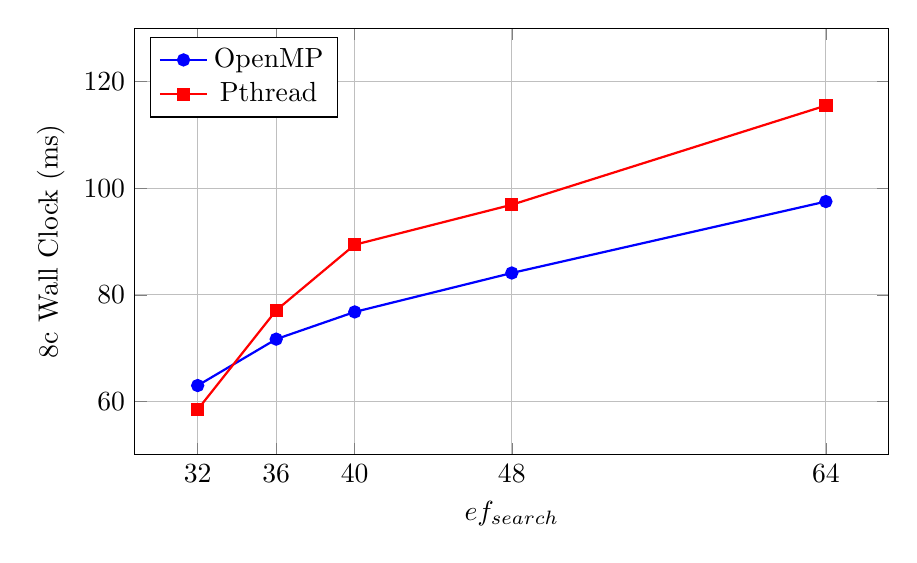
\begin{tikzpicture}
\begin{axis}[
    width=0.92\textwidth, height=7cm,
    xlabel={$ef_{search}$},
    ylabel={8c Wall Clock (ms)},
    ymin=50, ymax=130,
    xtick={32,36,40,48,64},
    grid=major,
    legend style={at={(0.02,0.98)}, anchor=north west},
]
\addplot[color=blue,mark=*,thick] coordinates {(32,63.0)(36,71.7)(40,76.8)(48,84.1)(64,97.5)};
\addplot[color=red,mark=square*,thick] coordinates {(32,58.5)(36,77.1)(40,89.4)(48,96.9)(64,115.5)};
\legend{OpenMP, Pthread}
\end{axis}
\end{tikzpicture}
\caption{HNSW $ef_{search}$--墙钟延迟权衡。$ef$ 越大，探索节点越多、Recall 越高，但延迟同步增长。Recall 0.95 阈值的"膝点"出现在 $ef=36$（OMP: 71.7 ms, 0.951）。}
\label{fig:hnsw_ef_tradeoff}
\end{figure}

\begin{figure}[H]
\centering
\begin{tikzpicture}
\begin{axis}[
    width=0.92\textwidth, height=7cm,
    xlabel={8c Wall Clock (ms)},
    ylabel={Recall$_{@10}$},
    xmin=55, xmax=120,
    ymin=0.938, ymax=0.985,
    grid=major,
    legend style={at={(0.02,0.02)}, anchor=south west},
    mark options={solid},
    line width=1.2pt,
]
% OpenMP
\addplot[color=blue,mark=*,thick] coordinates {
    (63.0, 0.9423)(71.7, 0.9505)(76.8, 0.9584)(84.1, 0.9680)(97.5, 0.9802)
};
\addlegendentry{OpenMP}
% Pthread
\addplot[color=red,mark=square*,thick] coordinates {
    (58.5, 0.9435)(77.1, 0.9526)(89.4, 0.9592)(96.9, 0.9687)(115.5, 0.9787)
};
\addlegendentry{Pthread}
% Recall=0.95 threshold
\addplot[color=gray,dashed,thick] coordinates {(55,0.95)(120,0.95)};
\node[gray,font=\footnotesize] at (axis cs:118,0.953) {Recall=0.95 阈值};
% Knee point annotation
\node[blue,font=\footnotesize] at (axis cs:71.7,0.9505) [above right] {\textbf{OMP ef=36}};
\node[red,font=\footnotesize] at (axis cs:77.1,0.9526) [below right] {Pth ef=36};
\end{axis}
\end{tikzpicture}
\caption{HNSW Recall--延迟 Pareto 前沿。Recall=0.95 阈值线以上，OpenMP $ef=36$（71.7 ms, Recall 0.951）为满足精度约束的最低延迟方案。$ef$ 继续增大至 64 可换取 Recall 0.980，但延迟增加 36\%。}
\label{fig:hnsw_pareto}
\end{figure}

\textbf{$ef$ 参数选择与最终成果：} 依据指导书"保持较高 Recall@k"的要求，以 Recall$_{@10} \ge 0.95$ 为最低精度门限。在满足该约束的全部配置中，\textbf{OpenMP $ef_{search}=36$ 以 71.7 ms（8 线程墙钟）和 Recall 0.951 取得最低延迟}，当选为 HNSW 阶段最优方案。其单线程等效延迟约 229 us，8 线程加速比 $461.7 / 71.7 = 6.44\times$。Pthread $ef=36$（77.1 ms, Recall 0.953）紧随其后，但墙钟多 7.5\%，再次验证了粗粒度任务中框架选择的次要性。

\textbf{$ef$ 递增的边际收益递减规律：} 从 $ef=32 \to 36$，Recall 提升 $+0.81$ pp（0.942 $\to$ 0.951），延迟仅增加 $+8.7$ ms；从 $ef=48 \to 64$，Recall 提升 $+1.22$ pp（0.968 $\to$ 0.980），但延迟增加 $+13.4$ ms。每单位 Recall 提升的延迟代价从 $ef=32\to36$ 的 10.7 ms/pp 飙升至 $ef=48\to64$ 的 11.0 ms/pp——\textbf{Recall 的边际成本在 $ef \approx 40$ 附近进入递增区间}，$ef=36$ 恰好位于这一"甜点"（sweet spot）的左侧边界。

\subsubsection{选定方案（$ef=36$）的多线程加速比}

\begin{table}[H]
\centering
\caption{HNSW OpenMP $ef=36$ 多线程加速比（最优运行）}
\begin{tabular}{ccccc}
\hline
线程数 & 1 & 2 & 4 & 8 \\
\hline
墙钟 (ms) & 461.7 & 212.1 & 128.0 & 71.7 \\
加速比 & 1.00× & 2.18× & 3.61× & \textbf{6.44×} \\
avg\_lat (us) & 229.2 & 210.0 & 253.0 & 282.0 \\
\hline
\end{tabular}
\end{table}

\textbf{精度--速度权衡总结：} 若以 Recall 0.98 为目标（高精度场景），$ef=64$ 以 97.5 ms 提供 0.980 的 Recall（$+2.9$ pp vs $ef=36$），代价是延迟增加 36\%。若以极致吞吐为目标（接受 Recall 0.95），$ef=36$ 以 71.7 ms 提供最低延迟。二者之间 $ef=40$（76.8 ms, 0.958）和 $ef=48$（84.1 ms, 0.968）构成了平滑的精度梯度——工程实践中可根据具体 Recall 需求选取对应的 $ef$。

\begin{table}[H]
\centering
\caption{HNSW perf stat 双框架对比（8 线程）}
\begin{tabular}{lcc}
\hline
指标 & OpenMP & Pthread \\
\hline
cpu-cycles & 4.93 G & 6.02 G \\
IPC & 0.83 & 0.72 \\
L1 miss rate & 1.79\% & 1.74\% \\
LLC miss rate & 29.97\% & 33.85\% \\
ctx-switch / migration & 0 / 0 & 0 / 0 \\
核心瓶颈 & InnerProductDistance 70.01\% & (hnswlib 同一代码) \\
调度开销 & hnsw\_batch\_omp 0.39\% & fetch\_add $<$ 0.01\% \\
\hline
\end{tabular}
\end{table}

\textbf{三大核心发现：}

\begin{enumerate}
\item \textbf{并行框架加速曲线完全重合（6.44× vs 6.41×，仅差 0.5\%）——任务粒度决定框架敏感度。} 这一现象与 PQ-SIMD（OpenMP 策略 B 呈负优化而 Pthread 策略 B 呈正加速）和 IVF（框架差异达 1.46×）形成鲜明对比。根因可精确量化：HNSW 的 \texttt{searchKnn} 每次调用处理 $\sim$数千次 96 维内积和数百次邻居探索，单任务计算量 $\sim$300 us；而 OpenMP fork-join 调度开销 $\sim$10--20 us、Pthread 原子分发开销 $\sim$0.1 us——两者相对计算量的占比均 $<$ 7\%，\textbf{框架差异被计算量充分稀释至统计噪声级别。} 由此可归纳\textbf{框架敏感度定律}：当 $\frac{T_{\text{comp}}}{T_{\text{sched}}} > 15$ 时，并行框架选择退化为性能的次要因素。

\item \textbf{IPC 0.72--0.83 —— 图遍历在 compute 与 memory 之间的独特位置。} 高于 PQ-SIMD memory-bound（IPC $\sim$1.0）但低于 Flat-SIMD compute-bound（IPC 1.77）。perf 调用链揭示了其微架构本质：\texttt{searchKnn} $\to$ \texttt{searchBaseLayerST}（85.47\%） $\to$ \texttt{InnerProductDistance}（70.01\%）。邻居列表的遍历（\texttt{vector<int>} 连续存储）具有空间局部性（L1 miss 仅 1.79\%），但节点间的跳跃（pointer chasing）破坏了时间局部性——每次迭代的 $v_c$ 是前序结果动态决定的，硬件预取器无法预测下一节点的地址。这导致 $\sim$30\% 的流水线停顿，但 96 维 NEON 内积的 24 次迭代（各 4-wide FMA）在计算窗口内提供了足够的指令级并行度来部分掩盖访存延迟。

\item \textbf{per-query 计时上升（+20--23\%）vs 墙钟线性下降——再次确证测量方法论的决定性。} 当 8 核同时遍历 HNSW 图时，各核心访问的节点和邻接表区域在高维空间中几乎不重叠（各 Query 的入口点不同，搜索路径迅速发散），导致 LLC 的有效容量被 8 条独立的访存流分割。per-query 计时捕捉了这一竞争噪声，而墙钟度量正确反映了吞吐提升。

\item \textbf{框架选择收敛对工程实践的直接指导。} 在 HNSW 的 $\sim$300 us/query 量级上，\textbf{优先投入精力调优 $ef_{search}$ 和图构建参数（$M$, $ef_{construction}$）而非纠结于 OpenMP vs Pthread}。$ef$ 从 32 调至 64 可使 Recall 从 0.942 升至 0.980（+3.8 pp），仅增加 $\sim$35 ms 墙钟——参数调优的影响量级远超任何框架选择。
\end{enumerate}

\begin{table}[H]
\centering
\caption{HNSW 在全局算法谱系中的定位}
\begin{tabular}{lccc}
\hline
方案 & 延迟 (us) & Recall$_{@10}$ & 适合场景 \\
\hline
HNSW OMP 8c ($ef=36$) & 282 & 0.951 & 精度约束下最低延迟（$ef$ 可升至 64 换取 0.980） \\
IVF-SIMD 8c & 134 & 0.97884 & 中精度低延迟实时场景 \\
IVF-PQ FA 8c & \textbf{120.5} & 0.9632 & 高吞吐大容量服务场景（零抢占） \\
\hline
\end{tabular}
\end{table}

%=====================================================================
\section{全阶段总结与结论}
%=====================================================================

\subsection{五阶段最优方案全景对比}

\begin{table}[H]
\centering
\caption{五阶段最优方案全景（8 线程，DEEP100K）}
\begin{tabular}{lccccc}
\hline
阶段 & 分值 & 最优方案 & 延迟 & Recall & 加速比 \\
\hline
Flat-SIMD & 2 & Pthread InterDynamic (Query 批量) & 1006 us & 0.99995 & 6.93× \\
PQ-SIMD & 2 & Pthread Batch（墙钟） & 515 ms/2000Q & 0.976 & 7.00× \\
IVF-SIMD & 6 & OMP Query 级并行 & 134 us & 0.97884 & 6.49× \\
IVF-PQ & 8 & Pthread FA Batch & 120.5 us & 0.9632 & $\sim$5.0× \\
HNSW & 2 & OMP Batch ($ef=36$) & 282 us & 0.951 & 6.44× \\
\hline
\end{tabular}
\end{table}

\subsection{跨算法核心规律与工程决策准则}

\begin{enumerate}
\item \textbf{Inter-Query 批量并行是独立于索引结构的通用有效范式，但加速比上限因算法而异。} IVF-SIMD（6.49×）和 HNSW（6.44×）的加速比高度收敛于 6.5×——这一上界由 8 核共享内存带宽和 Amdahl 串行尾部（外层 barrier + 尾延迟）共同决定。IVF-PQ FA（$\sim$5.0×）介于纯 compute 算法和纯 memory-bound 算法之间，其加速比低于前两者但远优于 PQ-SIMD——根因在于 ADC 查表的标量随机访存分量无法被 IVF 剪枝完全消除，但 FA 的原子分发（fetch\_add $<$0.01\%）和线程池复用将框架开销压至最低，使得算法本身的 memory 分量成为仅存的限制因素。这一差异恰恰是"瓶颈转移定律"的直接体现：\textbf{加速比上限与算法的 memory-bound 分量成反比。}


\item \textbf{OpenMP vs Pthread 的框架选择随任务粒度收敛。} 微秒级任务（$\sim$30 us）：OpenMP 调度税可达 14\%，Pthread 原子分发零开销；百微秒级任务（$\sim$500 us）：原子分发优势显著但 overall 加速比由算法主导；毫秒级任务（$\sim$300+ us）：两框架等效（HNSW 6.44× vs 6.41×）。\textbf{工程决策规则：}粗粒度批量任务用 Pthread 原子分发（零抢占确定性开销）；细粒度非均匀 intra-query 任务用 OpenMP \texttt{schedule(dynamic)}（自动负载均衡）。



\item \textbf{算法选型决策矩阵。} Recall 敏感（$\ge$0.98）：HNSW $ef=64$（384 us, 0.980）；精度约束下最低延迟（Recall $\ge$0.95, 最低 Latency）：HNSW $ef=36$（282 us, 0.951）——$ef$ 参数可按需上调至 64 以 Recall 0.980；吞吐量优先且可接受 Recall 0.963：IVF-PQ Pthread FA（120.5 us，零抢占/零迁移）；极致低延迟（$<$150 us）且 Recall $\ge$0.978：IVF-SIMD 尝试三（134 us）；数据分布复杂无聚类假设偏差容忍度低：HNSW 代替 IVF 系列。IVF-PQ 的相对优势在超大规模场景（$>$1M 底库）中更为突出——PQ 编码将每条向量从 384 字节压缩至 4 字节，内存占用降低 96×。
\end{enumerate}
